\section{A ring, eight anchors and a matching}\label{sec:ring}
Let $p\equiv1\pmod{840}$ be prime, $k\in\F^*$ a nonsquare, $H=\langle -1,3\rangle\subset\F^*$, $h=|H|$, $I=(p-1)/h$. Since $p\equiv1\pmod{12}$, both generators are squares. Call all board sites satisfying $xy=k$ modulo $p$ the \emph{carrier}, independently of any mask. By a \emph{fibre} we mean the set of points of the board reducing to one residue pair modulo $p$. The cosets $A$ and $k/A$ in $\F^*/H$ form distinct pairs: their quadratic characters differ. In each pair independently give one coset physical colour 0 and the other 1. For $u\ne0$ let $e(u)$ be the colour of its coset. Throughout the board $[0,4p]^2$, the fibre over $(u,k/u)$ has points $(x_0+ip,y_0+jp)$ with least positive representatives $x_0,y_0$ and $0\le i,j\le3$. Take the sites outside $\{1,2\}^2$ in sheet indices and having physical parity $x+y\equiv e(u)\pmod 2$. Thus $i+j\equiv e(u)-x_0-y_0\pmod 2$. Writing $ij$ for $(i,j)$, the two sheet masks are
\[
 M_0=\{00,02,13,20,31,33\},\qquad M_1=\{01,03,10,23,30,32\}.
\]
In $M_1$ the slopes to the other five sites, from $01$, $03$ and $10$ respectively, are
\[
 \{\infty,-1,1,-1/3,1/3\},\quad
 \{\infty,-3,0,-1,-1/3\},\quad
 \{-1,-3,3,0,1\}.
\]
The other three lists follow by the half-turn, and $(i,j)\mapsto(3-i,j)$ exchanges the masks. Thus each mask is a six-point cap, and the only primitive nonaxial directions in either mask, up to sign, are $(1,\pm1),(3,\pm1),(1,\pm3)$. A primitive physical line reduces to a genuine line modulo $p$ and meets $xy=k$ in at most two residues. Call the selected sites the \emph{ring points}, or old points. A triple of old points would therefore contain a same-fibre pair; all three cannot be in that fibre because its mask is a cap. An axis meets only one residue of the conic. For a nonaxial direction $(a,b)$ the other abscissa is $-ak/(bu)$ by the quadratic root product. Since $-a/b\in H$ for the listed directions, this lies in the coset paired with $uH$; its colour is opposite, whereas $x+y$ has constant parity on that physical line since $a+b$ is even. Thus every orientation gives a cap $O$ of size $6(p-1)$. The reflection in $C=(2p,2p)$ sends $u$ to $-u$, preserves parity and the outer sheets, so $O$ has the required half-turn. Call a coordinate \emph{coarse} if it is divisible by $p$. Every noncoarse physical row and column strictly inside $(p,3p)$ has exactly one old point: the two outer sheet choices in the other coordinate have opposite parities.

\paragraph{Boundary sites.} Add the eight anchors
\[B=p\{(0,1),(0,3),(1,0),(3,0),(4,1),(4,3),(1,4),(3,4)\}.\]
 These points are the eight extreme vertices of a convex octagon, so no three are collinear. From an anchor, a nonaxial primitive direction $(a,b)$ meets the carrier only at parameters satisfying $ab t^2=k\pmod p$. At height $\max(|a|,|b|)\le7$ every signed factor is a square modulo $p$ (use $p\equiv1\pmod{8}$ and quadratic reciprocity for $3,5,7$), so there are no such points. At height $D\ge8$ only the inward ray occurs, with $1\le t\le4p/D\le p/2$; it contains at most one of the two opposite roots modulo $p$ (and none if $p\mid ab$). A coarse axis misses the carrier. Lines between anchors have primitive height at most four. Thus $O\cup B$ is a cap for \emph{every} choice of the orientation bits.

Figure~\ref{fig:masks} shows what a change of colour means on an actual board: a bit exchanges the two masks in every fibre it controls. It neither moves the anchors nor changes the number of ring sites.
\begin{figure}[htbp]\centering
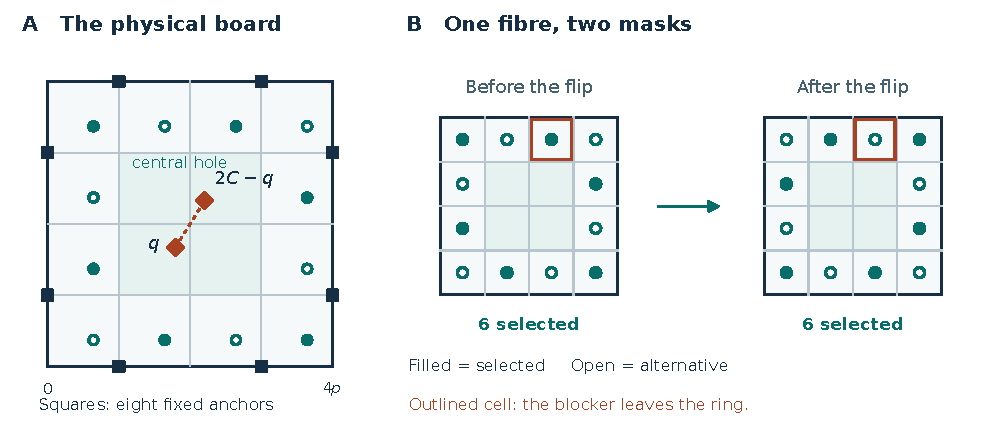
\includegraphics[width=.97\linewidth]{figures/ring-and-masks.pdf}
\caption{The mask switch at $p=73$, $k=28$. Left: only the twelve outer lifts of $(47,27)$ are drawn; the other fibres are omitted. The two diamonds are a proposed opposite pair, not ring sites. Right: the same fibre before and after the component flip. Cell $(2,3)$ contains $(193,246)$, an endpoint of the blocking secant through $q=(131,122)$ in Appendix~\ref{sec:finite}. Its removal costs no ring points in total. This finite illustration does not use the asymptotic sign test.}\label{fig:masks}
\end{figure}

\paragraph{Which pairs give clauses?} Fix the level $k$, but not the bits. Write $P_k$ for the union of the twelve outer-sheet sites over each $(u,k/u)$ (both masks together). Given one representative $q_i$ of each proposed opposite pair, form the list
\[
 \mathcal L_i=\big\{\{P,P'\}\subset P_k:\ P\ne P',\ q_i,P,P'\text{ collinear on a nonaxial integer line}\big\}.
\]
This is a list of \emph{unordered physical pairs}, not just of lines or of residue pairs. A line with $r$ possible sites contributes $\binom r2$ clauses, even if some pairs cannot be selected together by any orientation. The index $i$ is part of the clause identifier. An \emph{occurrence} is $(i,c,P)$ with $c\in\mathcal L_i$ and $P\in c$, and its label is
\[
 \lambda(i,c,P)=(P_x\bmod p)H\in\F^*/H.
\]
An endpoint used twice has two occurrences; it is not silently deduplicated. Its bit is indexed by the unordered coset pair $\{\lambda,k/\lambda\}$, not by $\lambda$ alone. Membership of $P$ asks that its coset receive its physical parity, so precisely one of the two bit values makes $P$ absent. The clause for $c$ asks that at least one of its two endpoints be absent.

\begin{lemma}[Matching all representatives]\label{lem:matching}
If the occurrence labels are pairwise distinct over the lists of all representatives, one orientation clears every listed pair both at the representatives and at their mates. Noncoarse central axes through a target already contain at most one selected ring point in every orientation.
\end{lemma}
\begin{proof}
Build the bipartite incidence graph from clauses to orientation bits. A bit has at most two occurrences in total, one per coset in its pair, even though two occurrences in one clause might refer to that same bit. Any $j$ clauses have exactly $2j$ occurrences, hence touch at least $j$ distinct bits. Hall's theorem~\cite{marriage} matches all clauses to distinct bits. For each clause set its assigned bit to disable one incident endpoint; no other clause asks to set that assigned bit. Set the unassigned bits arbitrarily. This precludes every potential pair that could give a triple with two selected ring points and a representative.

Let $R(P)=2C-P$. Reflection bijects $P_k$ with itself, preserves physical parity and sends the abscissa residue $u$ to $-u$, in the very same coset since $-1\in H$. Thus a reflected clause has the same two membership requirements, not two additional occurrences for the degree count. At a central noncoarse physical row or column the one-site observation above handles an axis directly. The two partner cosets of a single bit may both occur.
\end{proof}

Figure~\ref{fig:match} illustrates why the distinction between a coset and a bit matters. The two clauses have four distinct endpoint cosets, but just two orientation bits between them. Each clause is assigned a different one.
\begin{figure}[htbp]\centering
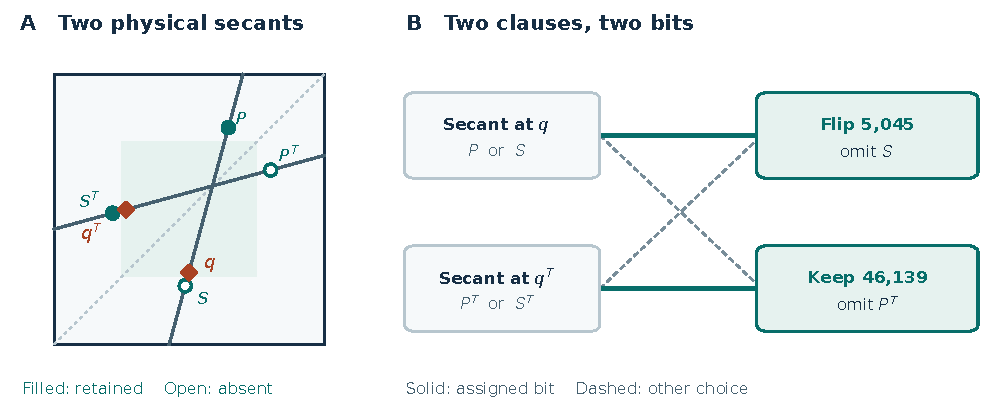
\includegraphics[width=.97\linewidth]{figures/matched-secants.pdf}
\caption{Part of the certified $p=797\,161$ matching. The two representatives are $q$ and its \emph{transpose} $q^T$, not half-turn mates. The secant at $q$ has endpoints $P=q+155653(3,11)$ and $S=q-14051(3,11)$; transposing the coordinates gives the other secant. A solid edge assigns its clause a bit, labelled by its least component residue. Flipping bit $5045$ disables $S$; retaining bit $46139$ leaves $P^T$ absent. The left panel shows these final choices. Reflection then protects the two mates as well.}\label{fig:match}
\end{figure}

\section{Sampling opposite pairs at one level}\label{sec:sampling}
Choose one level $k\in\F$ uniformly. Independently of it, sample $N$ independent uniform residues $z_i=(X_i,Y_i)\in\F^2$. Index $i$ proposes the two actual sites $q_i=(p+[X_i]_p,p+[Y_i]_p)$ and $2C-q_i$, where $[\ ]_p\in[0,p-1]$. We call $q_i$ the representative and $z_i$ its root modulo $p$. Write $d_i=X_iY_i$ and let $\ch$ be the quadratic character, zero at zero. We now define a test $E_i$ for \emph{one} index and show $\Prob(E_i)\ge\gamma>0$ for all sufficiently large $p$, with absolute $\gamma$. We will use linearity of expectation, not an assumption that these tests at the shared level are independent.

First require $\ch(d_i)=+1$ and $\ch(k)=-1$. For each primitive $(a,b)$ with $a>0$, $ab\ne0$, $\max(|a|,|b|)\le8$ require
\begin{equation}\label{eq:shortslope}
 \ch(k-\rho_{i,a,b})=-1,\qquad \rho_{i,a,b}=-(aY_i-bX_i)^2/(4ab).
\end{equation}
The discriminant of $(X_i+at)(Y_i+bt)=k$ is $4ab(k-\rho_{i,a,b})$, and $4ab$ is a square. In these directions no carrier point lies on the line, even before a mask is chosen.

Consider two carrier endpoints at signed offsets $t,u$ from $q_i$ along a primitive direction. Divide $t,u$ by their common gcd; the larger of the two resulting absolute values is the \emph{ratio height}. The next identity is the two-endpoint discriminant underlying fixed barycentric weights; compare~\cite{ratioante}. To exclude ratio heights at most 8, require $\ch(k-d_i)=-1$ and
\begin{equation}\label{eq:shortratio}
 \ch(k-\beta d_i)=+1\quad(\beta\in\R),\qquad
 \R=\left\{\left(\frac{r-s}{r+s}\right)^2:\ 0<|r|,|s|\le8,\ r\ne\pm s\right\}.
\end{equation}
Indeed let the reduced parameters be $r,s$, and $(U,V)$ the first endpoint modulo $p$. The second is $(1-s/r)z_i+(s/r)(U,V)$. The offsets are nonzero modulo $p$ because $k\ne d_i$. When the reduced parameters have height at most eight, $r-s\ne0$ modulo all $p>16$ since the endpoints are distinct. Both endpoints have product $k$; expanding and cancelling $r-s$ shows that $s(Y_iU+X_iV)=(r+s)k+(s-r)d_i$, whence
\[
 [s(Y_iU-X_iV)]^2=(k-d_i)\big((r+s)^2k-(r-s)^2d_i\big).
\]
For $r+s\ne0$ the right side is a nonsquare by \eqref{eq:shortratio}; for $r+s=0$ its second factor is $-4r^2d_i$, a square since $\ch(-1)=\ch(d_i)=1$. The first factor is still a nonsquare, so this too is impossible. The same protections hold for the reflected root.

\begin{lemma}[The finite sign prescription]\label{lem:signs}
At one representative the test uses exactly 130 shifted signs of the level, in addition to the test on $d_i$. For all sufficiently large primes in the progression its unconditional probability is bounded below by an absolute constant $\gamma>0$.
\end{lemma}
\begin{proof}
The following count gives a reproducible deduplication without a long list of fractions. There are $\sum_{v=2}^8\varphi(v)=1+2+2+4+2+6+4=21$ reduced fractions $u/v$ with $1\le u<v\le8$. Positive primitive ordered pairs in the $8$-box number $1+2\cdot21=43$ (include $(1,1)$); the two signs of $b$ give 86 slopes for $a>0$. For each of the 21 proper fractions include in $\R$ exactly
\[
 \left(\frac{v-u}{v+u}\right)^2\quad\text{and its reciprocal}.
\]
These are precisely the ratio shifts in~\eqref{eq:shortratio}: common scaling and interchanging $r,s$ leave the square unchanged, while changing one sign inverts it. The first values are strictly between zero and one and are distinct since $(1-z)/(1+z)$ is strictly decreasing there; their reciprocals exceed one. Thus there are 42, none equal to $0$ or $1$.

For an indeterminate root $(X,Y)$, the 130 shift polynomials are $0$, $XY$, the 42 polynomials $\beta XY$, and the 86 polynomials
\[
 -\frac{b}{4a}X^2+\tfrac12 XY-\frac{a}{4b}Y^2.
\]
The last group has nonzero $X^2$ coefficients distinguishing the signed slopes $b/a$; the first three groups have zero $X^2$ coefficient and distinct $XY$ coefficients. Distinctness over $\mathbb Q$ therefore follows before any root or level is chosen. Only finitely many primes divide a denominator or all nonzero numerators of a coefficient difference. Outside them the shift polynomials stay distinct in $\F[X,Y]$. Each difference has total degree at most two and vanishes on at most $2p$ pairs $(X,Y)$ (the elementary polynomial zero bound). The probability that any two \emph{values} coincide is at most $2\binom{130}{2}/p$. Also $\Prob(\ch(XY)=1)=(p-1)^2/(2p^2)$. Hence a positive fraction, tending to $1/2$, of roots pass the latter condition and have no coincident values.

Fix such a root and write $\mathcal A=\{a_1,\ldots,a_s\}$ for its distinct shifts, $s=130$. Put $\epsilon_j=-1$ for $0,XY$ and the 86 direction shifts, and $\epsilon_j=+1$ for the 42 ratio shifts. For every $k\in\F$ put
\[
  \mathcopy{P(k) = 2^(-s) product_{j=1}^s (1 + epsilon_j chi(k - a_j)).}{P(k)=\prod_{j=1}^{s}\frac{1+\epsilon_j\ch(k-a_j)}{2}.}
\]
For $k\notin\mathcal A$, this is the indicator that all signs agree. At a shift value the sign prescription fails, since $\ch(0)=0$. On $\mathcal A$ one factor of $P(k)$ is $1/2$ and every other factor is at most one. Thus
\[
  \mathcopy{R_A = sum_{k in A} P(k), with 0 <= R_A <= s/2.}{R_{\mathcal A}:=\sum_{k\in\mathcal A}P(k),\qquad 0\le R_{\mathcal A}\le s/2.}
\]
Writing $[s]=\{1,\ldots,s\}$, the number $N_z$ of admissible levels at this root is exactly
\[
\mathcopy{N_z = sum_{k in F_p} P(k) - R_A = p/2^s + 2^(-s) sum_{nonempty J in powerset([s])} (product_{j in J} epsilon_j) sum_{k in F_p} chi(product_{j in J} (k - a_j)) - R_A.}{\begin{aligned}
  N_z&=\sum_{k\in\F} P(k)-R_{\mathcal A}\\
     &=\frac{p}{2^s}
       +\frac{1}{2^s}\sum_{\varnothing\ne J\subseteq[s]}
         \left(\prod_{j\in J}\epsilon_j\right)
         \sum_{k\in\F}\ch\!\left(\prod_{j\in J}(k-a_j)\right)
       -R_{\mathcal A}.
\end{aligned}}
\]
Each nonempty $J$ gives a product of distinct linear factors. The Weil bound~\cite[Theorem 5.41]{weil} bounds its character sum by $(|J|-1)\sqrt p$ in absolute value. Consequently
\[
  \mathcopy{|N_z - p/2^s| <= (1 - 2^(-s)) (s-1) sqrt(p) + s/2.}{\left|N_z-\frac{p}{2^s}\right|
  \le (1-2^{-s})(s-1)\sqrt p+\frac{s}{2}.}
\]
For sufficiently large $p$, at least $1/4$ of the roots have the required $\ch(XY)$ and distinct shifts, and for each of them $N_z/p\ge 2^{-131}$. Multiplication gives $\Prob(E_i)\ge 2^{-133}$. This is a marginal bound for $(z_i,k)$, not a conditional bound given the tests at other roots.
\end{proof}

\paragraph{Other types of triples.} We record costs according to the number of distinct sampled indices involved.
\begin{itemize}
\item For one index on $E_i$, a line through a target and an anchor, or through the two mates, reduces to the line through zero of slope $Y_i/X_i$, a square. Thus it misses $xy=k$. The two coordinates of each target are noncoarse, strictly inside $(p,3p)$, and the mates use different rows and columns. A target on an anchor--anchor line, or an anchor on the line between mates, costs $O(1/p)$ per index: in the latter case the representative is on the fixed line from $C$ to the anchor.
\item For two distinct indices and any choice of signs, condition on their two target positions. Off the diagonal the joining line has $O(1+p/D)$ board sites if its primitive height is $D$. Each site is on the carrier with probability $1/p$ over the independent uniform $k$. For a fixed first site and a uniform second site in its translated $p$-square, there are $O(D)$ primitive directions of height $D$, each containing $O(1+p/D)$ choices. Thus the off-diagonal mean of $1/D$ is at most $O(p^{-2})\sum_{D\le4p} D(1+p/D)/D=O(L_p/p)$. By summing the $1/p$ site probabilities, the joining-line cost is $O(1/p+\mathbb E[\mathbf{1}_{\rm distinct}/D])=O(L_p/p)$ per pair of indices. Coincidences, shared rows or columns, a joining line through an anchor, or a third target that is the mate of one of the first two, cost $O(1/p)$ per pair. Indeed a line contains at most $p$ sites in a translated $p$-square. For an anchor test fix the first target off the anchor, then expose the second site. A target coinciding with the fixed anchor costs at most $1/p^2$ even without eligibility. For a mate triple condition on its opposite pair first.
\item For three distinct indices, any three-target collinearity costs $O(1/p)$ per triple of indices: choose signs and condition on two distinct positions (coincidences are already marked). There are only eight sign choices.
\end{itemize}
These are unconditional upper bounds for bad events, with eligibility imposed where stated; they are not used as conditional probabilities after the character test. After resolving them only triples with two old points and one target still require work.

\section{Encoding the remaining secants}\label{sec:encoding}
For one root $z=(x,y)$ (residue of $q$), write a physical chord as the ordered template $g=(a,b,t,u)$, with primitive $(a,b)$, $a>0$, $b\ne0$, $t<u$, and actual offsets $t(a,b),u(a,b)$ from $q$. Each coordinate of an offset has absolute value at most $4p$. We count a superset of the actual chords by using this coordinate bound and dropping all outer-sheet and window restrictions. On $E_i$ surviving physical chords at $q_i$ have both direction and ratio height greater than 8. They satisfy $p\nmid abtu(t-u)$: $p\mid t$ or $p\mid u$ would put $z$ on the carrier; if $p\mid(t-u)$ for an actual board chord, its endpoint difference has length at least $p$ times the direction height in the infinity norm, so that height is at most four. If $p\mid ab$, the modular line is axial and gives only one residue, again forcing $p\mid(t-u)$. Axial physical lines have already been handled.

The offsets relative to $q$ determine its physical unordered endpoint pair uniquely; a chosen endpoint order will cost at most two. Conversely every pair in $\mathcal L_i$ at a passing representative yields one of these canonical generic templates.

For such a template, incidence of both endpoints with $xy=k$ is equivalent to
\begin{equation}\label{eq:hit}
 k-xy=-abtu,\qquad bx+ay=-ab(t+u).
\end{equation}
Subtracting the endpoint equations first gives $(u-t)(bx+ay+ab(t+u))=0$. Substitution gives the first identity as well; this is the rooted calculation of~\cite[\S2]{root} with the level uniform in all of $\F$. For each $x$ the second equation determines $y$ and the first determines $k$: there are exactly $p$ hits among $p^3$ outcomes before restricting the level. A specified template therefore hits with probability $p^{-2}$. Two templates at the same root with distinct modular slopes require equal products $abtu=a'b't'u'$ in $\F$; if so, their equations fix $x,y,k$ uniquely. Their joint probability is $p^{-3}$. We only count collisions for $k\ne0$ and nonzero endpoint abscissas.

Split direction height into dyadic bins $D\le\max(|a|,|b|)<2D$. Then $|a|,|b|\le 2D$ and $|t|,|u|\le T=\lfloor4p/D\rfloor$, where $DT\asymp p$ for $1\le D\le4p$. There are $O(D^2)$ choices of direction and $O(T^2)$ choices of parameters, hence $O(p^2)$ templates per bin and $O(p^2L_p)$ in total. In the same template the endpoint abscissas $x+at,x+au$ are distinct. The value $e=1$ is impossible. For each other $e\in H$, the equation $x+au=e(x+at)$ has at most one $x$; $y,k$ then follow from \eqref{eq:hit}. Hence a collision between the two slots of a single template costs $O(p^2 L_p\,h/p^3)=O(hL_p/p)$ per root.

\section{Two chords through the same representative}\label{sec:one}
A \emph{generic template} below has the nonvanishing conditions of Section~\ref{sec:encoding} and the four integer bounds $|at|,|au|,|bt|,|bu|\le4p$. These constraints are imposed before taking probabilities. The canonical order is $t<u$; when an endpoint is designated for comparison we may temporarily put its parameter first. All upper counts below allow either parameter order. A \emph{hit} means that both endpoints reduce to the level $k$; they need not be selected by a mask. Throughout this section the random experiment has exactly $p^3$ equally likely outcomes $(x,y,k)$. We count on $k\ne0$ and $xy\ne k$ where required; that restriction does not decrease the denominator.

\subsection{Equal modular slopes: counting distinct physical lifts}
\begin{lemma}[Parallel lifts]\label{lem:lifts}
The probability that two distinct generic physical chords of direction and ratio heights greater than eight both hit the same nonzero level at one root and have equal modular slopes is $O(L_p/p)$.
\end{lemma}
\begin{proof}
The two modular lines through the root coincide. Each chord has two distinct endpoint residues ($a(u-t)\ne0$), and the conic has at most two intersections with that line. Reorder the second chord's two columns to align these residues. For the two matrices of \emph{integer offsets} we then have
\begin{equation}\label{eq:liftmat}
 M=v(t,u),\quad v=(a,b)^{\mathsf T},\qquad M'=M+pE,\quad |E_{ij}|\le8.
\end{equation}
Each difference is a multiple of $p$ by the column alignment, and $|E_{ij}|=|M^{\prime}_{ij}-M_{ij}|/p\le(4p+4p)/p=8$, independently of the direction bin. If $E=0$, the physical unordered endpoints agree, hence so do the canonical templates. Thus $E\ne0$. This reasoning includes the possibility that different pairs lie on the very same ordinary line.

If $E$ has rank one, write $E=rs^{\mathsf T}$ over $\mathbb Q$. Then $M+pE=[v\ r]\operatorname{diag}(1,p)[(t,u)^{\mathsf T}\ s]^{\mathsf T}$. Its determinant is zero, so either $r$ is parallel to $v$ or $s$ is parallel to $(t,u)^{\mathsf T}$. In the first case a nonzero column of $E$ is an integer multiple of the primitive vector $v$; in the second a nonzero row is an integer multiple of the primitive row $(t,u)/\gcd(|t|,|u|)$. In either case the corresponding height is at most eight, contrary to hypothesis. This is the point at which the short \emph{ratio} exclusion is needed in addition to the short-direction exclusion.

Suppose now that $E$ is invertible. Write $d=\gcd(|t|,|u|)$ and $w=(t,u)^{\mathsf T}/d$. Both $v$ and $w$ are primitive. With $J=\operatorname{adj}(E)$, expanding the determinant in~\eqref{eq:liftmat} gives
\begin{equation}\label{eq:bilin}
 0=p^2\det E+pd\,w^{\mathsf T}Jv,
 \qquad d\mid |\det E|.
\end{equation}
Indeed $d\mid p\det E$ and $p\nmid d$ by genericity. Each of the four entries has 17 possible integer values, so the entire box contains exactly 83,521 matrices, including the singular ones. Of these, 81,152 are nonsingular by direct enumeration; only the uniform upper bound is needed. For a nonsingular choice, $1\le |\det E|\le 8\cdot8+8\cdot8=128$.

Here is the integer-point count for fixed $E,d$. In a bin $D\le\norm v<2D$ we have $\norm w\le U=4p/(dD)$; if $U<1$ there are no solutions. For fixed primitive $v$, write $c=Jv$ and $g=\gcd(|c_1|,|c_2|)$. Then $c\ne0$, and $g\mid |\det E|$ because $Ec=(\det E)v$ and the entries of $v$ are coprime. The same identity gives $\norm c\ge |\det E|\norm v/16$ (each absolute row sum of $E$ is at most 16). If the equation $c\cdot w=-p\det E/d$ is soluble, its integer solutions form one progression with primitive step $(c_2,-c_1)/g$. Indeed the kernel of the primitive row $c/g$ in $\mathbb Z^2$ is generated by that step. Its infinity norm is $\norm c/g\ge\norm v/16$. If $c_1=0$, the second coordinate of a solution is fixed and the step is $(\pm1,0)$; if $c_2=0$ it is $(0,\pm1)$. Both coordinates cannot vanish. Intersecting a progression of step $s$ with $[-U,U]^2$ gives at most $1+\lfloor 2U/\norm s\rfloor$ points by looking along its largest coordinate. Thus the bound holds also on the axes.

If $D\le U$, each of the $O(D^2)$ choices of $v$ contributes $O(1+U/D)$ points in the $w$-box. The product is $O(D^2+DU)=O(p)$. If $U<D$, fix primitive $w$ first. Apply the same argument to $J^{\mathsf T}w$ and $E^{\mathsf T}$: for $\norm w=m$ the number of possible $v$ in the larger box is $O(1+D/m)$. The integer square has $8m$ points of norm exactly $m\ge1$, so the bin contributes at most
\[
 \sum_{m\le U}8m\,O(1+D/m)=O(U^2+DU)=O(p).
\]
Here $DU=4p/d$. For each solution, $M$ and $M'=M+pE$ are fixed. A nonzero rank-one $M'$ admitting a second template determines its primitive direction with positive first coordinate, and then its two parameters, up to the column order we temporarily allowed. Thus each solution yields at most two ordered representations of the second chord (one in canonical order). Summing the $O(L_p)$ bins and the finitely many $E,d$ gives $O(pL_p)$ pairs, with absolute constants. By~\eqref{eq:hit} the first template alone hits with probability $p^{-2}$. The union bound proves the assertion.
\end{proof}

\subsection{Unequal modular slopes: a divisor count and a direction count}
Let two templates have distinct modular slopes. Designate one endpoint of each for comparison, and relabel so their signed parameters are $t,t'$ (not necessarily the lesser parameters). Write $U=x+at$, $V=x+au$, $U'=x+a't'$ for three endpoint abscissas. In a joint hit at $xy\ne k\ne0$ no two of the residues on distinct lines can agree: the only intersection of the lines is the root, which is not on the conic. Distinct conic residues have both coordinates distinct. The slope between abscissas $s_1,s_2$ on the conic is $-k/(s_1s_2)$. Dividing the slope from $U$ to $V$ by the slope from $V$ to $U'$ therefore gives
\[
 \frac{U'}{U}=\frac{b}{a}\frac{a't'-au}{b't'-bu}
 =\frac{\alpha-\lambda}{\beta-\lambda},\qquad
 (\alpha,\beta,\lambda,\mu)=\left(\frac{a'}a,\frac{b'}b,\frac{u}{t'},\frac{t}{u'}\right).
\]
All divisions here are in $\F$ by nonzero elements. If these two occurrences share a coset, $e=U'/U\in H$. Equality of the products in~\eqref{eq:hit} and the last identity give the two necessary conditions
\begin{equation}\label{eq:ABCD}
 \alpha\beta=\lambda\mu,\qquad \alpha-e\beta=(1-e)\lambda.
\end{equation}
Here $e\ne1$, since otherwise $\alpha=\beta$ and the slopes are equal. We will count using only necessary conditions, not assert that each counted pair is a chord on the board.

\begin{lemma}[Four large gcds]\label{lem:gcd}
Let $G\ge1$ be an integer. Among ordered generic template pairs with
$abtu\equiv a'b't'u'\pmod p$, the number for which at least one of
\[
 \gcd(a,a'),\quad\gcd(b,b'),\quad\gcd(u,t'),\quad\gcd(t,u')
\]
is greater than $G$ is $O(p^3 L_p^5/G)$. Gcds are positive and taken in $\Z$.
\end{lemma}
\begin{proof}
In a specified row of the following table, fix any common divisor $\ell>G$ of the indicated two factors. Since both are nonzero modulo $p$, $p\nmid\ell$. The table writes the two products \emph{after cancelling the same} $\ell$ in $\F$. Each row still has the congruence $ij\equiv i'j'\pmod p$.
\begin{center}\small
\begin{tabular}{@{}ccccc@{}}\toprule
Factors divisible by $\ell$ & $i$ & $j$ & $i'$ & $j'$ \\ \midrule
$a,a'$ & $(a/\ell)t$ & $bu$ & $(a'/\ell)t'$ & $b'u'$\\
$b,b'$ & $(b/\ell)t$ & $au$ & $(b'/\ell)t'$ & $a'u'$\\
$u,t'$ & $a(u/\ell)$ & $bt$ & $a'(t'/\ell)$ & $b'u'$\\
$t,u'$ & $a(t/\ell)$ & $bu$ & $a'(u'/\ell)$ & $b't'$\\ \bottomrule
\end{tabular}\end{center}
In each row $0<|i|,|i'|\le 4p/\ell$, $0<|j|,|j'|\le4p$, by the four offset bounds on each template. None of the four products vanishes modulo $p$. For fixed $i,j$ there are at most $4\tau(|i|)\tau(|j|)$ choices of the original four factors: choose the magnitude of the first factor as a positive divisor and choose its sign; the signed second factor is then forced. Thus there are exactly $2\tau(|i|)$ signed splittings for the $i$-column and $2\tau(|j|)$ for the $j$-column. Their two factor slots are disjoint in each row, and the indicated slot, not an arbitrary one, is multiplied back by $\ell$. The primed columns work the same way. Ignoring primitivity, sign conventions and the physical window only increases this bound.

For fixed $i,i'$ put $c=i/i'\in\F^*$ and group $j$ by its residue. With
\[
 W(r)=\sum_{0<|j|\le4p,\ j\equiv r\ (p)}\tau(|j|)\quad(r\in\F^*),
\]
the sum of the remaining weights is $\sum_r W(r)W(cr)\le\sum_r W(r)^2$, by Cauchy--Schwarz and the permutation $r\mapsto cr$. Each residue has at most nine integer representatives in $[-4p,4p]$. A second Cauchy--Schwarz, now within each residue, gives
\[
 \sum_r W(r)^2\le 18\sum_{m\le4p}\tau(m)^2\ll pL_p^3.
\]
For the last inequality, $\tau(m)^2\le d_4(m)$ by multiplicativity and $(j+1)^2\le\binom{j+3}{3}$ at a prime power. Counting four positive factors by fixing the first three gives $\sum_{m\le X}d_4(m)\le X(1+\log X)^3$ for $X\ge1$. Similarly $\sum_{m\le X}\tau(m)\le X(1+\log X)$. Applying the latter bound to both signed small factors $i,i'$ costs $O((p/\ell)^2L_p^2)$. If $4p/\ell<1$ the count is zero. Otherwise the cost for this row and divisor is $O(p^3L_p^5/\ell^2)$. Every bad pair occurs for at least its gcd, so summing over the four rows and $\sum_{\ell>G}\ell^{-2}\le1/G$ proves the lemma. This is a global count; no dyadic-bin factor is charged in it.
\end{proof}

\begin{lemma}[One modular ratio in a rectangle]\label{lem:ratio}
For $c\in\F^*$, $S,T>0$ and an integer $G\ge1$, the number of integer pairs with $0<|s|\le S$, $0<|t|\le T$, $p\nmid st$, $t\equiv cs\pmod p$ and $\gcd(|s|,|t|)\le G$ is
\begin{equation}\label{eq:ratio}
 O(G+ST/p),
\end{equation}
uniformly in all parameters.
\end{lemma}
\begin{proof}
There is nothing to count if $S<1$ or $T<1$. First require primitivity. Representatives of one rational direction then consist of at most a vector and its negative. Two different rational directions have a nonzero integer determinant divisible by $p$. After scaling the coordinates by $1/S,1/T$, the absolute determinant is at least $p/(ST)$ and each vector has Euclidean norm at most $\sqrt2$. Write the directions as angles modulo $\pi$. If there are at least two, each consecutive cyclic gap $\theta$ lies in $(0,\pi)$ and satisfies
\[
  \sin\theta\ \ge\ \frac{p}{2ST}.
\]
If $2ST<p$ this is impossible. At $2ST=p$ every gap would be $\pi/2$, so there are at most two directions. For $p/2<ST<p$ a single direction is not forced, but each gap exceeds $1/2$ radian. In general, summing $\theta\ge\sin\theta\ge p/(2ST)$ around the circle gives at most $2\pi ST/p$ directions whenever there are two or more. Including the empty and singleton cases and both signs, the primitive-pair count is at most $2+4\pi ST/p$.

For gcd \emph{exactly} $j$ write $(s,t)=j(s_0,t_0)$ with $(s_0,t_0)$ primitive. If $p\mid j$ there are no admissible pairs. Otherwise cancellation of $j$ gives the same congruence in the box of radii $S/j,T/j$. These gcd classes are disjoint, so the total is at most
\[
  \sum_{\substack{1\le j\le G\\p\nmid j}}
       \left(2+\frac{4\pi ST}{p\,j^2}\right)
  \le 2G+\frac{8\pi ST}{p}.
\]
This proves~\eqref{eq:ratio}.
\end{proof}

\begin{proposition}[Nonparallel collision at one root]\label{prop:nonparallel}
For $1\le G\le\sqrt p$ integral, the probability of a joint hit of two generic templates of unequal modular slopes with a common designated endpoint coset, at a nonzero level off the root, is
\begin{equation}\label{eq:nonparallel}
 O\left(\frac{L_p^5}{G}+\frac{h}{p}(1+G)^2 L_p^2\right).
\end{equation}
The event is the existence of such a pair, with any endpoint order.
\end{proposition}
\begin{proof}
For a fixed nonparallel pair the two linear equations in $x,y$ in~\eqref{eq:hit} are independent. If the products agree, there is one solution and then one value of $k$; otherwise no outcome works. Thus Lemma~\ref{lem:gcd}, divided by $p^3$, bounds the contribution of large gcds even without enforcing the coset ratio.

For the remaining pairs fix two direction bins $D,D_1$ with parameter bounds $T=\lfloor4p/D\rfloor$, $T_1=\lfloor4p/D_1\rfloor$. Put $X=DD_1$ and $Y=TT_1$. Since $2p\le DT,D_1T_1\le4p$, we have
\begin{equation}\label{eq:binsize}
 4p^2\le XY\le16p^2.
\end{equation}
If $X\ge p$, choose the four signed parameters in $O(T^2T_1^2)=O(Y^2)$ ways and choose $e$ in at most $h$ ways. Then $\lambda,\mu$ are fixed, and~\eqref{eq:ABCD} gives
\[
 e\beta^2+(1-e)\lambda\beta-\lambda\mu=0,\qquad \alpha=e\beta+(1-e)\lambda.
\]
Its leading coefficient is nonzero, so there are at most two pairs $(\alpha,\beta)$. For each, realize $a'/a=\alpha$ and $b'/b=\beta$ separately in boxes of radii $2D,2D_1$. Each has $O(G+4X/p)$ possibilities by Lemma~\ref{lem:ratio}. Multiplying these upper bounds does not presume independence: retaining all combinations only overcounts. The number in these bins is at most
\[
 O\big(hY^2(G+X/p)^2\big)\ll h(1+G)^2(XY/p)^2\ll h(1+G)^2p^2.
\]
If $X<p$, choose both directions in $O(D^2D_1^2)=O(X^2)$ ways, and choose $e\in H\setminus\{1\}$. The first two ratios are fixed. Now $\lambda=(\alpha-e\beta)/(1-e)$ is unique; zero is inadmissible, and otherwise $\mu=\alpha\beta/\lambda$ is unique as well. Realize $u/t'=\lambda$ and $t/u'=\mu$ in the two boxes with radii $T_1,T$, with gcds at most $G$. The number is at most
\[
 O\big(hX^2(G+Y/p)^2\big)\ll h(1+G)^2(XY/p)^2\ll h(1+G)^2p^2,
\]
since $Y\ge p$ by~\eqref{eq:binsize}. For clarity about multiplicity, the two chords are \emph{ordered}; each belongs to one bin $D=2^j$ and $0\le j\le\lfloor\log_2(4p)\rfloor$. The primitive direction with $a>0$ is unique. On each chord either of its two physical endpoints can be designated; these two choices just interchange the two parameters. Thus at most $2\cdot2$ designations and $(1+\lfloor\log_2(4p)\rfloor)^2$ ordered bin pairs cover every comparison. The counts allowing both parameter orders already overcount some of them. This bounds the small-gcd total by $O(h(1+G)^2p^2L_p^2)$. Each fixed nonparallel pair specifies at most one residue root and level, hence at most one physical representative under the prescribed lift. Dividing by $p^3$, then adding the large-gcd term, gives~\eqref{eq:nonparallel}.
\end{proof}

\section{Two roots at the same level}\label{sec:two}
\begin{proposition}[Cross-root collision]\label{prop:cross}
For two independently sampled representatives and one shared random level, the probability that a generic hit at the first representative and a generic hit at the second have a common designated endpoint coset at $k\ne0$ is
\[
 O\big(L_p^2(h/p+p^{-1/2})\big).
\]
The bound is unconditional; it also bounds the event with either or both sign tests imposed.
\end{proposition}
\begin{proof}
Fix two templates and a designation of endpoints. Let $m=b/a$, $m'=b'/a'$, $\Delta=u-t$, $\Delta'=u'-t'$, all nonzero in $\F$. If the first designated abscissa is $U$, then the other abscissa on the first line is $U+a\Delta$, and the slope formula gives
\begin{equation}\label{eq:levelU}
 k=-mU(U+a\Delta).
\end{equation}
For a common coset write $U'=eU$ with $e\in H$. Equate~\eqref{eq:levelU} to $-m'eU(eU+a'\Delta')$ and divide by $U\ne0$:
\begin{equation}\label{eq:crosslin}
 (m-e^2m')U=e b'\Delta'-b\Delta.
\end{equation}
Given a solution $U$, equation~\eqref{eq:levelU} determines $k$. The two roots are uniquely recovered as $(U-at,k/U-bt)$ and $(eU-a't',k/(eU)-b't')$. If the left coefficient in~\eqref{eq:crosslin} is nonzero there is at most one $U$; if only the right side is nonzero there is none. In these nonexceptional cases there are $O(p^4L_p^2)$ ordered template pairs and at most $h$ ratios. Each contributes at most one of the $p^5$ equiprobable outcomes $(k,x,y,x',y')$, not one of $p^6$: the level is shared. This gives $O(hL_p^2/p)$.

In the exceptional case \emph{both} sides of~\eqref{eq:crosslin} vanish identically in $U$. As $b'\Delta'\ne0$, necessarily
\begin{equation}\label{eq:exception}
 e=\frac{b\Delta}{b'\Delta'},\qquad ab\Delta^2=a'b'(\Delta')^2\ne0.
\end{equation}
The second equation follows by substituting the first into $b/a=e^2 b'/a'$. Conversely the second forces that coefficient to vanish for this unique ratio. If the ratio is not in $H$, discard the pair; in particular there is \emph{no factor $h$} in counting exceptional pairs.

For fixed first template let $c=ab\Delta^2$. In one bin $(D_1,T_1)$ there are two bounds on the number of second templates satisfying the invariant in~\eqref{eq:exception}:
\begin{enumerate}
\item Choose $(a',b')$ in $O(D_1^2)$ ways. The congruence $(\Delta')^2=c/(a'b')$ has at most two roots. For each of $O(T_1)$ choices of $t'$, the residue of $u'=t'+\Delta'$ has at most nine representatives in $[-T_1,T_1]$, since $T_1\le4p$. Cost: $O(D_1^2 T_1)$.
\item Choose $(t',u')$ in $O(T_1^2)$ ways with $\Delta'\ne0$ modulo $p$, then $a'$ in $O(D_1)$ ways. The residue $b'=c/(a'(\Delta')^2)$ is unique and has at most 17 representatives in $[-2D_1,2D_1]$, since $D_1\le4p$. Cost: $O(D_1 T_1^2)$.
\end{enumerate}
The smaller bound is $O(D_1T_1\min(D_1,T_1))=O(p^{3/2})$ because $D_1T_1\le4p$. For each exceptional pair there are at most $p-1$ nonzero values of $U$, each specifying at most one whole outcome by the reconstruction above. The union bound, including the choice of first template, second bin, and outcome, is therefore
\[
 \frac{O(p^2 L_p)\,O(L_p)\,O(p^{3/2})\,(p-1)}{p^5}
 =O(p^{-1/2}L_p^2).
\]
Endpoint order costs only an absolute factor. There is no use of independence between mates: their clauses were identified by symmetry in Lemma~\ref{lem:matching}.
\end{proof}


\section{Choosing a compatible subfamily}\label{sec:choose}
\begin{lemma}[Exhaustion of ordinary triples]\label{lem:triples}
Suppose the retained proposals pass the sign test, all the one-, two- and three-index geometric exceptions of Section~\ref{sec:sampling} have been removed, and an orientation clears the lists $\mathcal L_i$ of the representatives. Then the union of the ring, the eight anchors and the retained opposite pairs is a cap.
\end{lemma}
\begin{proof}
Write $O$ for a selected ring point, $B$ for an anchor and $T$ for either sign of a retained target. The sets are disjoint: anchors are coarse, ring points are noncoarse, and eligible targets are noncoarse and off the carrier. An eligible index supplies two distinct sites, and coincidences between indices have been marked. The table lists every multiset of three site types; entries concern three \emph{distinct physical points}.
\begin{center}\small\renewcommand{\arraystretch}{1.13}
\begin{tabularx}{\linewidth}{@{}lX@{}}\toprule
Types & Reason a triple of these types cannot survive \\ \midrule
$OOO$ & Same-fibre pair, mask and opposite coset colour (Section~\ref{sec:ring}).\\
$OOB$ & A line from an anchor contains at most one carrier site: the short-direction square test or the inward-ray bound (Section~\ref{sec:ring}).\\
$OBB$ & An anchor--anchor axis is coarse; a nonaxis anchor--anchor line has primitive height at most four and misses the carrier.\\
$BBB$ & All eight anchor sites are extreme vertices.\\
$OOT$ & The central axes have only one old site each; every nonaxial pair is a clause, including at the mate by reflection (Lemma~\ref{lem:matching}).\\
$OBT$ & The target--anchor line reduces to the square-slope line through zero and misses the nonsquare level.\\
$BBT$ & Reject an index with either site on one of the finitely many anchor--anchor lines.\\
$OTT$ & Mates give the same square-slope exclusion. For different indices mark a joining line with any carrier site, for every choice of signs.\\
$BTT$ & For mates reject the index if its diameter contains an anchor. For different indices mark the pair if the joining line contains an anchor.\\
$TTT$ & With two indices, a mate pair determines a diameter and a third site on it marks the pair of indices. With three indices mark signed three-site collinearity. One index has only two sites.\\ \bottomrule
\end{tabularx}\end{center}
These ten multisets exhaust the possibilities. In particular the test for three independent indices does not stand in for a test on two sites of one opposite pair.
\end{proof}

\begin{proposition}\label{prop:index} For all sufficiently large primes $p\equiv1\pmod{840}$ with $I\ge L_p^{24}$, the number of opposite pairs that can be added to a suitably oriented anchored ring is
\[
 \gg \frac{\min(I,\sqrt p)}{L_p^3}.
\]
\end{proposition}
\begin{proof} Use $G=\max(1,\lfloor I^{1/4}\rfloor)$ in \eqref{eq:nonparallel}. Call an index \emph{eligible} if it passes $E_i$, has no one-index geometric exception and all endpoint occurrences of its nonaxial blocking secants through the representative use distinct $H$-cosets. On $E_i$ these are among our generic, long-direction, long-ratio templates. Removing impossible outer-sheet points from the template count can only help. Any two occurrences belong to the two slots of one chord, two different chords at one representative (equal or unequal modular slopes), or two different representatives. Reuse of a physical endpoint is included in this partition. The last case is a two-index event. For the within-root cases use Section~\ref{sec:encoding}, Lemma~\ref{lem:lifts} and Proposition~\ref{prop:nonparallel}, respectively. Let $B_i$ denote failure of any of the additional one-index checks. Since $h/p\le I^{-1}$ and $G\asymp I^{1/4}$, their unconditional costs give
\begin{equation}\label{eq:one}
\mathcopy{Pr(E_i and B_i) << (1+L_p)/p + L_p/I + L_p^5/I^(1/4) + L_p^2/sqrt(I) << L_p^5/I^(1/4) <= 1/L_p for I >= L_p^24.}{\begin{aligned}
 \Prob(E_i\cap B_i)
 &\ll \frac{1+L_p}{p}+\frac{L_p}{I}
       +\frac{L_p^5}{I^{1/4}}+\frac{L_p^2}{\sqrt I}\\[2pt]
 &\ll \frac{L_p^5}{I^{1/4}}\le \frac{1}{L_p},
 \qquad I\ge L_p^{24}.
\end{aligned}}
\end{equation}
Hence the mean number of eligible indices among $N$ proposals is at least $\gamma N/2$. The shared level is not resampled.

Mark an edge on two eligible indices for any two-index geometric exception, or if blocking endpoints at their representatives use a common $H$-coset. By Proposition~\ref{prop:cross} and the geometric estimates, the cost for a specified pair of indices is
\begin{equation}\label{eq:two}
  \Prob\big(\{i,j\}\text{ is marked}\big)
    \ll L_p^2\!\left(\frac{1}{I}+\frac{1}{\sqrt p}\right).
\end{equation}
Also mark a three-index edge for a collinearity among three eligible indices, at probability $O(1/p)$ for each triple. Put $J=\min\{I,\sqrt p\}$ and $N=\lfloor J/L_p^3\rfloor$. Then $N\to\infty$ under the index hypothesis. For the total number $Z$ of marked edges,
\[
  \mathcopy{E[Z] << N^2 L_p^2/J + N^3/p << N/L_p + N/L_p^6 = o(N).}{\mathbb E Z
   \ll \frac{N^2 L_p^2}{J}+\frac{N^3}{p}
   \ll \frac{N}{L_p}+\frac{N}{L_p^6}=o(N).}
\]
Here $N/J\le L_p^{-3}$ and $N^2/p\le L_p^{-6}$. Subtracting, for some outcome the number of eligible indices minus the number of marked edges is at least $\gamma N/4$. Choose one index in each marked edge and discard the union of the chosen indices (Figure~\ref{fig:pruning}). The union has size at most $Z$. This leaves at least $\gamma N/4$ indices with no marked edges. Their level is nonsquare because each passed $E_i$.

All blocking endpoint occurrences in the surviving representatives now have distinct $H$-cosets, both within and across indices. Lemma~\ref{lem:matching} chooses one orientation that disables every such secant, and by symmetry the same is true at all the mates. Lemma~\ref{lem:triples} now excludes every ordinary triple. Thus the $6(p-1)$ chosen old points, the eight anchors and all the retained opposite pairs form one half-turn cap, with no restriction on direction. Changing an orientation swaps six sites for six in each affected fibre. Thus each retained opposite pair accounts for two net additional points.
\end{proof}

\begin{figure}[htbp]\centering
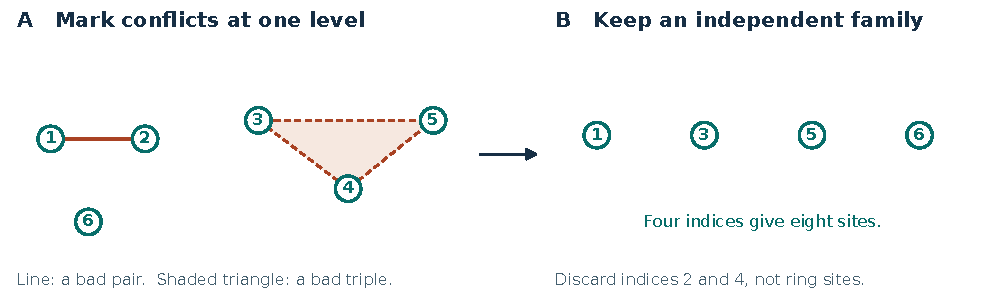
\includegraphics[width=.97\linewidth]{figures/shared-level-selection.pdf}
\caption{How the deletion step in Proposition~\ref{prop:index} works, schematically. Each numbered vertex is one eligible index at the \emph{same} level $k$ and represents two opposite sites. Meeting the marked pair and the marked triple removes every indicated conflict. The matching is performed on the survivors. The diagram illustrates the deletion rule, not observed conflict frequencies.}\label{fig:pruning}
\end{figure}

\section{The cyclotomic choice of primes}\label{sec:primes}
\begin{proof}[Proof of Theorem~\ref{thm:main}] Apply Stewart's theorem \cite[Theorem 1, (7)]{stewart} to $\Phi_j(3,1)$ for large multiples $j$ of 840. Here $(3+1)^2=16$ and $3\cdot1=3$ are coprime nonzero integers, and $3/1$ is not a root of unity. The largest prime divisor satisfies
\[
 p> j\exp\!\left(\frac{\log j}{104\log\log j}\right).
\]
As $p>j$, $X^j-1=\prod_{d\mid j}\Phi_d(X)$ is separable modulo $p$. Its cyclotomic factors therefore share no root. Since $3$ is a root of $\Phi_j$ modulo $p$, its multiplicative order is exactly $j$. Thus $p\equiv1\pmod{840}$; moreover $j$ is even, $-1\in\langle3\rangle$, and $h=j$. Distinct orders give distinct primes. For all sufficiently large primes so obtained,
\[
 \log I\ge \frac{\log p}{210\log\log p}:
\]
if $j\le\sqrt p$ this is immediate, while if $j>\sqrt p$, Stewart gives $\log(p/j)>\log p/(208\log\log p)$. Passing to $I=(p-1)/j$ adds $\log(1-1/p)$, absorbed by replacing 208 with 210. In particular $I\ge L_p^{24}$ eventually. Also $\sqrt p\ge \exp(\log p/(210\log\log p))$ eventually. By Proposition~\ref{prop:index}, the log of the number of extra points is therefore at least
\[
 \frac{\log p}{210\log\log p}-3\log L_p-O(1)
 \ \ge\ \frac{\log p}{300\log\log p}
\]
for all sufficiently large primes in this sequence. This gives~\eqref{eq:main}. For a prescribed integer $m$, one may also keep exactly $m$ of the supplied opposite pairs on all sufficiently large boards of the sequence.\end{proof}

The constant 300 is not optimized. Neither a conjecture about multiplicative orders nor empirical independence of secants is used. The proof supplies no numerical cutoff at which one can expect the character prescription to become practical: there are 130 simultaneous signs, and only their fixed number is used in the asymptotic argument.
